\item \points{1d}

Consider a website that wants to predict its daily traffic. The website owners have collected a dataset of past traffic to their website, along with some features which they think are useful in
predicting the number of visitors per day. The dataset is split into train/valid sets and the starter code is provided in the following files:
\begin{center}
    \begin{itemize}
        \item 	\texttt{src-poisson/{train,valid}.csv}
        \item   \texttt{src-poisson/submission.py}
    \end{itemize}
\end{center}
We will apply Poisson regression to model the number of visitors per day. Note that applying Poisson regression in particular assumes that the data follows a Poisson distribution whose natural parameter is a linear combination of the input features (\emph{i.e.,} $\eta = \theta^T x$). In \texttt{src-poisson/submission.py}, implement Poisson regression for this dataset and use \emph{full batch gradient ascent} to maximize the log-likelihood of $\theta$. For the stopping criterion, check if the change in parameters has a norm smaller than a small value such as $10^{-5}$. Please complete the |fit| and |predict| functions of the |PoissonRegression| class. 

Using the trained model, predict the expected counts for the \textbf{validation set}.  To verify a correct implementation, use autograder test case |1d-2-basic| to create a scatter plot between the true counts vs predicted counts (on the validation set). In the scatter plot, the x-axis is the true count and the y-axis are the corresponding predicted expected count. Note that the true counts are integers while the expected counts are generally real numbers.\\

Your plot should look similar to the following:

\begin{figure}[H]
	\centering
	\vspace{-2mm}
	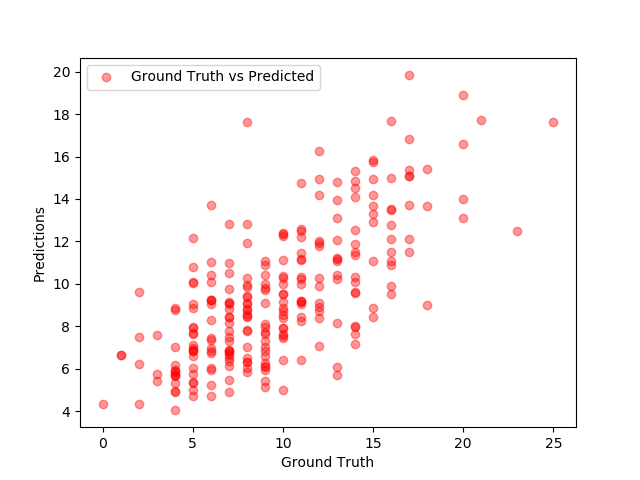
\includegraphics[width=0.65\linewidth]{01-poisson/poisson_val.png}
	\caption{Ground Truth vs Prediction plot on the validation set (Note: This is for reference only.  You are not required to submit a plot.)}
\end{figure}